% $Id: introduction.tex 1784 2012-04-27 23:29:31Z nicolas.cardozo $
% !TEX root = main.tex

\chapter{The back-in-time debugger in depth}
\label{cha:indepth}

This section explains how the back-in time debugger works internally. The basic building block for the way the debugger get to accomplish what it does, is by means of enforcing programmers to use the MVI architectural pattern for their code, using a server to store all the states that have happened during the execution of the program and using a client (Intellij plugin) to let users interact with the previously mentioned features.

The code of this project is available at \url{https://github.com/af-orozcog/MVIKotlin}.

\section{The MVI architectural pattern and MVIKotlin}

Having based the back-in-time debugger on an existing project, it is necessary to first introduce the concepts used by the original project to use logging and time travel functionalities, as those are still needed to use the new plugin. But the focus would only be in the necessary pieces of information needed to test the back-in-time new plugin. For more information refer to \url{https://arkivanov.github.io/MVIKotlin/}

\subsection{MVI}

MVI which stands for Model-View-Intent is an architectural pattern characterized for the flow of data in an unidirectional way. Flow of data from the model to the view and from the view to the model. A simple schema of the model can be viewed in the next figure.

\begin{figure}[h]
\centering
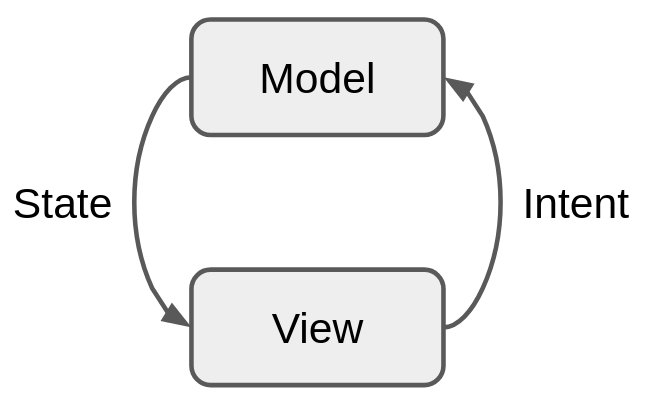
\includegraphics[height=3cm,width=4cm]{figures/mvi}
\caption{Sample MVI pattern (Ivanov, n.d.)}
\label{fig: Sample MVI pattern}
\end{figure}

\subsection{MVIKotlin}

Is the Kotlin multiplatform framework that lets programmers write shared code using MVI and which is necessary to be able to use the back-in-time features.

\subsubsection{Core components and responsibility}

\begin{itemize}
   \item \textbf{Store}: which represents the Model from the MVI, this is the place where the business logic should be placed. This is where the single source of the \textbf{State} is defined and stored.
  	\item \textbf{MviView}: which represents the View from the MVI, is preferably the place where UI logic takes place, but this component is optional.
\end{itemize}

\subsubsection{The flow of the data}

The following figure shows a conventional way of how the data should flow between components:

\begin{figure}[h]
\centering
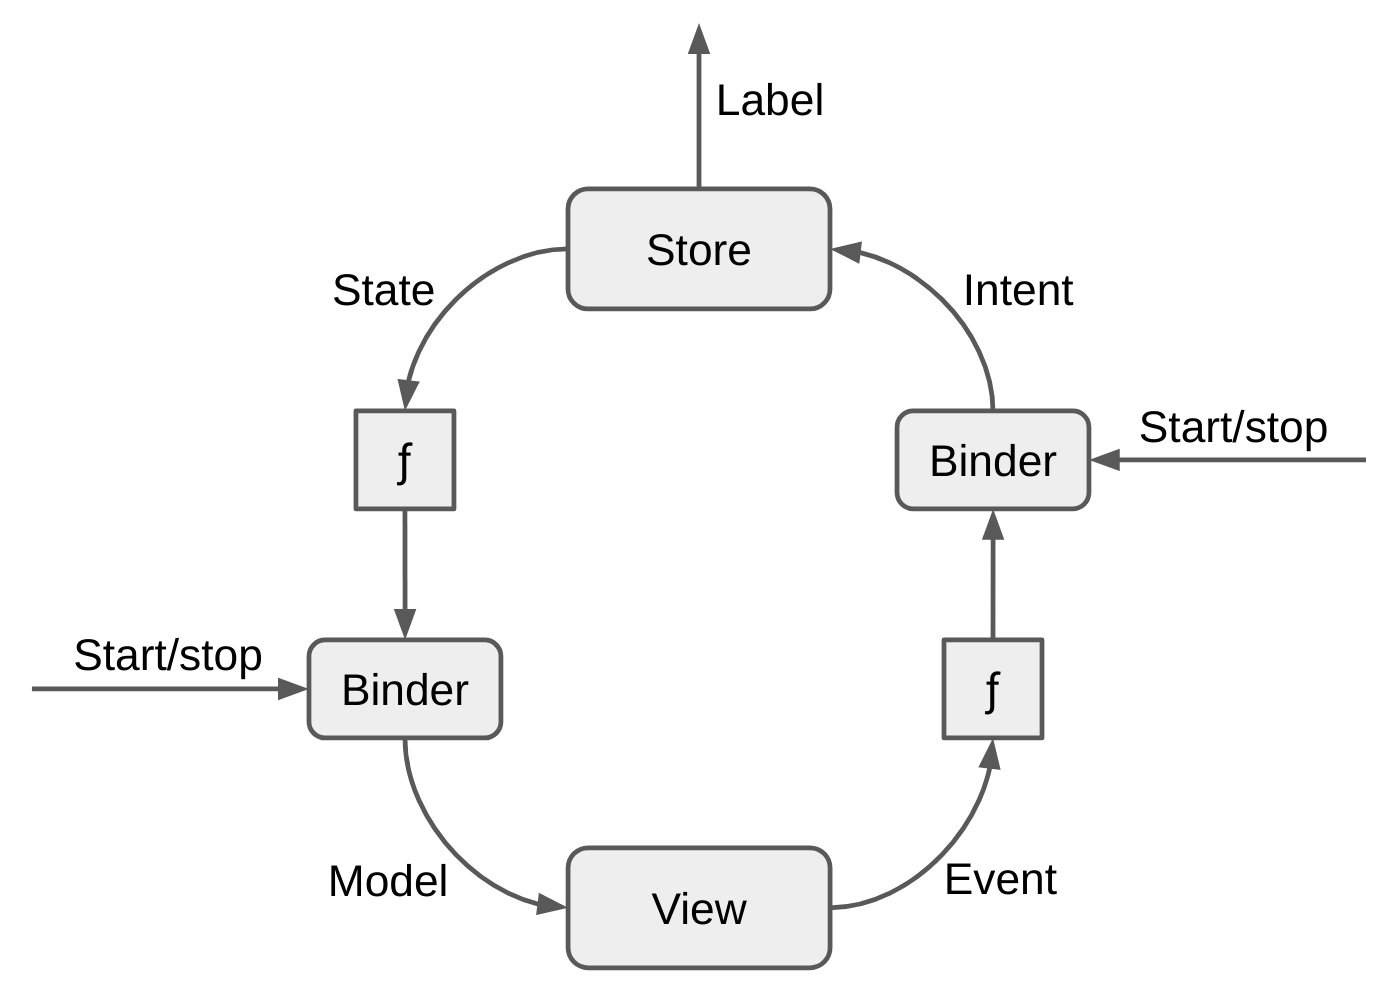
\includegraphics[height=5cm,width=7cm]{figures/flowdata}
\caption{Sample flow of data MVIKotlin (Ivanov, n.d.)}
\label{fig: Sample flow of data MVIKotlin}
\end{figure}

The \textbf{store} would generate a stream of states which are in turn translated to a series of view models by means of a function \textbf{f}, these views can be digested and used by the \textbf{view}.

The \textbf{view} would generate a stream of events which are in turn also translated into intents by a function \textbf{f}, these intents can be digested by the \textbf{store} that then updates its state.

\subsubsection{Store}
The \textbf{store} is the place where business logic is placed. Its structure is shown in the following figure:

\begin{figure}[h]
\centering
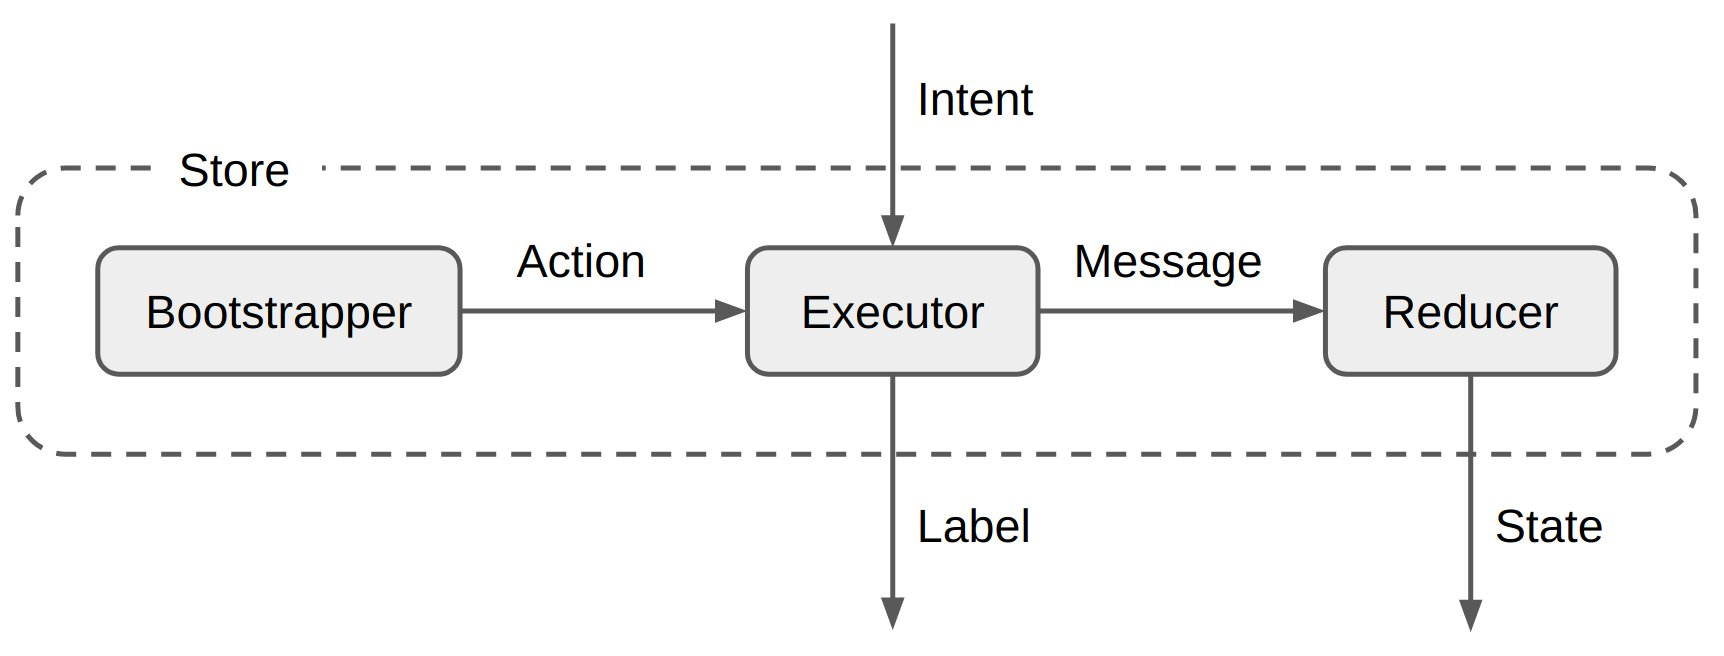
\includegraphics[height=5cm,width=7cm]{figures/storeStructure}
\caption{Store structure (Ivanov, n.d.)}
\label{fig: Store structure}
\end{figure}

\begin{itemize}
   \item \textbf{Bootstrapper}: This component kick-starts the \textbf{store}. If it is passed to the \textbf{storeFactory}, it will produce \textbf{actions} that are consumed by the \textbf{executor} at some point in the creation of the \textbf{store}.
  	\item \textbf{Executor}: This is the place where all the business logic takes place, asynchronous operations might be added here. It receives messages to process in the form of \textbf{intents} and \textbf{actions} from the outside world and from the \textbf{bootstrapper}, respectively. It also has outputs of the form of \textbf{labels} and \textbf{messages}. \textbf{Messages} are received in the \textbf{reducer} and \textbf{labels} are dispatched to the outside world. Here the operations to update the \textbf{state} are performed, but the outcome is sent to the \textbf{reducer}.
  	\item \textbf{Reducer}: This component receives \textbf{messages} from the \textbf{executor} and according to them updates the current \textbf{state} of the \textbf{store}, and emits this update to observers of the \textbf{state} changes.
\end{itemize}

It is possible to define your own \textbf{store}, but for most use cases, including the \textbf{store} needed for time traveling, the built-in \textbf{storeFactories} will be enough. The following is a piece of code adapted from \url{https://arkivanov.github.io/MVIKotlin/store.html}, it defines a \textbf{store} to represent a counter.

\lstset{
 columns=fullflexible,
 frame=single,
 breaklines=true,
 postbreak=\mbox{\textcolor{red}{$\hookrightarrow$}\space},
}

\begin{lstlisting}[language=java]
internal interface CalculatorStore : Store<Intent, State, Nothing> {

   sealed interface Intent {
       object Increment : Intent
       object Decrement : Intent
       data class Sum(val n: Int): Intent
   }

   data class State(
       val value: Long = 0L
   )
}

internal class CalculatorStoreFactory(private val storeFactory: StoreFactory) {

	private sealed interface Msg {
       class Value(val value: Long) : Msg
   }

	private sealed interface Action {
       class Sum(val n: Int): Action
   }

   fun create(): CalculatorStore =
       object : CalculatorStore, Store<Intent, State, Nothing> by storeFactory.create<Intent, Action, Msg, State, Nothing>(
           name = "CounterStore",
           initialState = State(),
           bootstrapper = coroutineBootstrapper {
               launch { // Launch a coroutine
                   val sum = withContext(Dispatchers.Default) { (1L..1000000.toLong()).sum() }
                   dispatch(Action.SetValue(sum)) // Dispatch an Action
               }
           },
           executorFactory = coroutineExecutorFactory {
               // Register a handler for Action.SetValue
               onAction<Action.SetValue> { action ->
                   dispatch(Msg.Value(action.value)) // Read the Action and dispatch a Message
               }

               // Register a handler for Intent.Increment
               onIntent<Intent.Increment> {
                   dispatch(Msg.Value(state.value + 1)) // Read the current state and dispatch a Message
               }

               onIntent<Intent.Decrement> { dispatch(Msg.Value(state.value - 1)) }

               onIntent<Intent.Sum> { intent ->
                   launch { // Launch a coroutine
                       val sum = withContext(Dispatchers.Default) { (1L..intent.n.toLong()).sum() }
                       dispatch(Msg.Value(sum))
                   }
               }
           },
           reducer = { msg ->
               when (msg) {
                   is Msg.Value -> copy(value = msg.value)
               }
           }
       ) {
       }
}

\end{lstlisting}

In order to create a \textbf{store}, as seen in the previous example, the programmer must provide a definition of the \textbf{intents}, \textbf{actions}, \textbf{messages} and \textbf{labels} the \textbf{store} receives or sends from and to the outside world. In addition, the developer must create the \textbf{bootstrapper}, \textbf{executor} and \textbf{reducer}, components that react to the different events happening during the execution of the program.

\section{Server-client architecture for recording states}

\subsection{Server}

After the developer has defined the \textbf{store(s)} and state(s) of the program that will be recorded through the execution of it, they will need to be created using the time travel \textbf{storeFactory}. Once all the previous steps have been done, the coder must start the time travel server, which will save all the \textbf{stores} and all the \textbf{actions}, \textbf{labels}, \textbf{intents} and \textbf{messages} that are generated during the execution of the program. This can be done as shown in the following piece of code for mobile development:

\begin{lstlisting}[language=java]
class App : Application() {
   private val timeTravelServer = TimeTravelServer()

   override fun onCreate() {
       super.onCreate()
       timeTravelServer.start()
   }
}
\end{lstlisting}
And as follows for JVM app development
\begin{lstlisting}[language=java]
fun main() {
   TimeTravelServer(runOnMainThread = { SwingUtilities.invokeLater(it) })
       .start()
}
\end{lstlisting}

\subsubsection{How it works}

The time travel server works by keeping track of all the \textbf{stores} created using the time travel \textbf{storeFactory}, and subscribing to all events being sent or received to these \textbf{stores}. Once an event is sent to a \textbf{store} or created by it, it is first processed in the time travel server by adding it to a list of events, and then forwarding it to the corresponding \textbf{store} to react to it.

Notice that events generated or received by \textbf{stores} are usually of type \textbf{intent}, \textbf{action} or \textbf{label}. But both the time travel \textbf{store} and server will process events of new type called \textbf{state}, this type of event will record the moment the state changes after the reducer has processed the event of type \textbf{message}, while also storing the new state of the store.

Events of type \textbf{state} are of special importance, because they enable the time travel server to define what it means to move either forward or backwards in states that have happened chronologically. This is because the server can easily identify how the state of a store should change. This is specially important because \textbf{intents} and \textbf{messages} cannot generally be used to retrieve the previous state of a given \textbf{store}.

\subsubsection{Commands and connection to the Intellij plugin}

Besides storing the events and \textbf{store} objects the server can receive commands from the Intellij plugin to perform actions such as moving backwards or forward in the changes of the states of the program and reflect the changes in the UI, in case an UI component is connected to the \textbf{stores} that are being updated. These commands are received over the internet, in the case of mobile applications the adb is used to be able to send these commands.

Besides moving forward and backwards, the server would also receive commands to be able to investigate what happened in a specific event. This process involves receiving the id of the event to investigate from the Intellij plugin, but also sending the specific event parsed back to the plugin, for doing that the events need to be parsed before being sent over the network, this is done with the help of the custom library proto-internal, which is used always before reading or writing to the network.

\section{Additions to MVIKotlin}

The proposed solution to be able to change events in the past, specially those concerning the state of a \textbf{store}, is to expose a series of functions in the \textbf{store} that when called will generate an \textbf{intent}. \textbf{Intents} are afterall the only events that can trigger the change of the state of a \textbf{store}.

Two new problems arise, how are those functions going to be called from the Intellij plugin and how are they going to be exposed. For these problems, the solution was to modify the interface of the \textbf{stores} to include two new attributes.

\begin{itemize}
   \item \textbf{exposedFunctionsSignature}: This new variable holds the signature of the functions that can be called. It specifies the parameters of the function and a short description that can easily be parsed and sent over the network from the server to the Intellij plugin. Following is the attribute definition in the \textbf{store} interface, which makes developers at least take into account its existence, because it enforces them to define at the very least an empty TimeTravelFunctionList:
  
\begin{lstlisting}[language=java]
/**
* Returns the functions and the signatures
*/
val exposedFunctionsSignature:TimeTravelFunctionList
\end{lstlisting}
	\item \textbf{exposedFunctions}: This is a map of strings to functions, functions that all receive a list of any type that will be the parameters sent from the Intellij plugin, this makes it easier to serialize the parameters over the network. Although only a couple of variable types are available to be serialized now, like strings and integers. Following is the attribute definition in the \textbf{store} interface:
\begin{lstlisting}[language=java]
/**
* the actual functions that a user can call
*/
var exposedFunctions:Map<String,(arguments:List<Any>) -> Unit>
\end{lstlisting}
\end{itemize}

These two elements give all the necessary tools for developers to expose the changes that they want to be able to trigger in the state of a \textbf{store}, effectively changing the state of an event that happened in the past.

\section{Additions to the time travel server}

Given that the user now is able to change the events that have happened in the past and "re-run" the program from there on, while also letting it check previous executions events. The main changes are as follows:

\begin{itemize}
	\item Serializer and deserializer for functions calls: new functions were added to be able to parse function signatures from the server to the Intellij plugin, and to parse functions arguments from the Intellij plugin to the server.
	\item Events list of lists: Given that the objective was to let developers check all previous execution events, a list of lists was created to reflect all execution events.
	\item Handlers for functions and events: Now that users are also able to change events in the past, handlers for functions that trigger \textbf{intents} must be added. Specially a modification in which events are handled was specially important. Given that modifying a state in the past is equivalent to starting from it. New methods had to be defined to go backwards in time just before the modifying function of the state is triggered and then add the subsequent events to a new list of events that starts from the modified state.
\end{itemize}

\section{Additions to the Intellij plugin}

\begin{figure}[h]
\centering
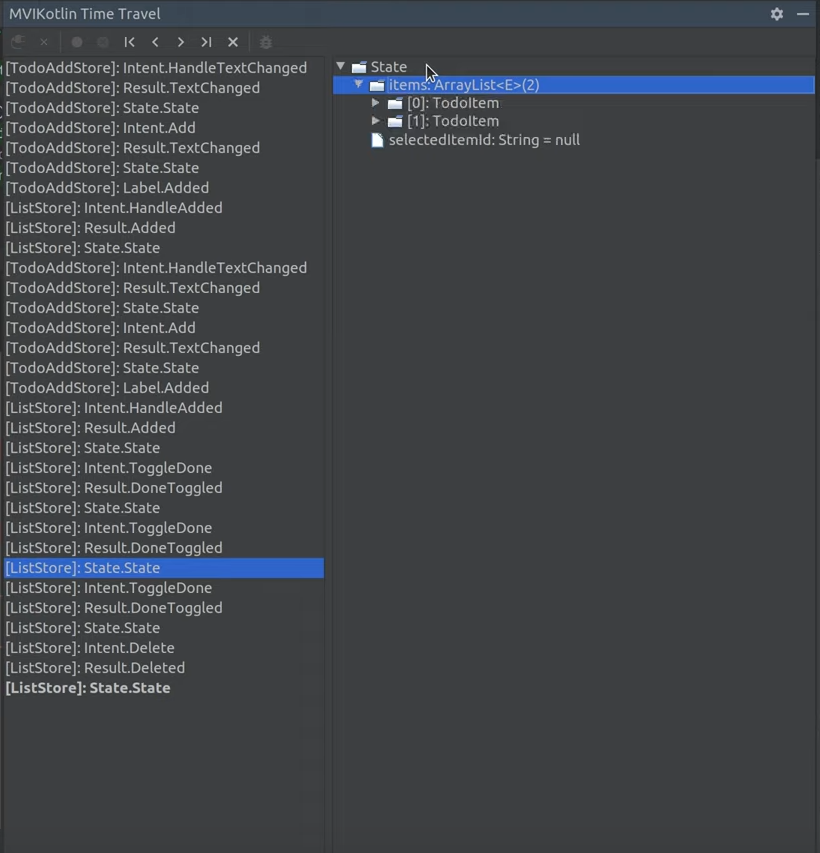
\includegraphics[height=6cm,width=10cm]{figures/oldPlugin}
\caption{Sample view of the old plugin}
\label{fig: Sample view of the old plugin}
\end{figure}

\begin{figure}[h]
\centering
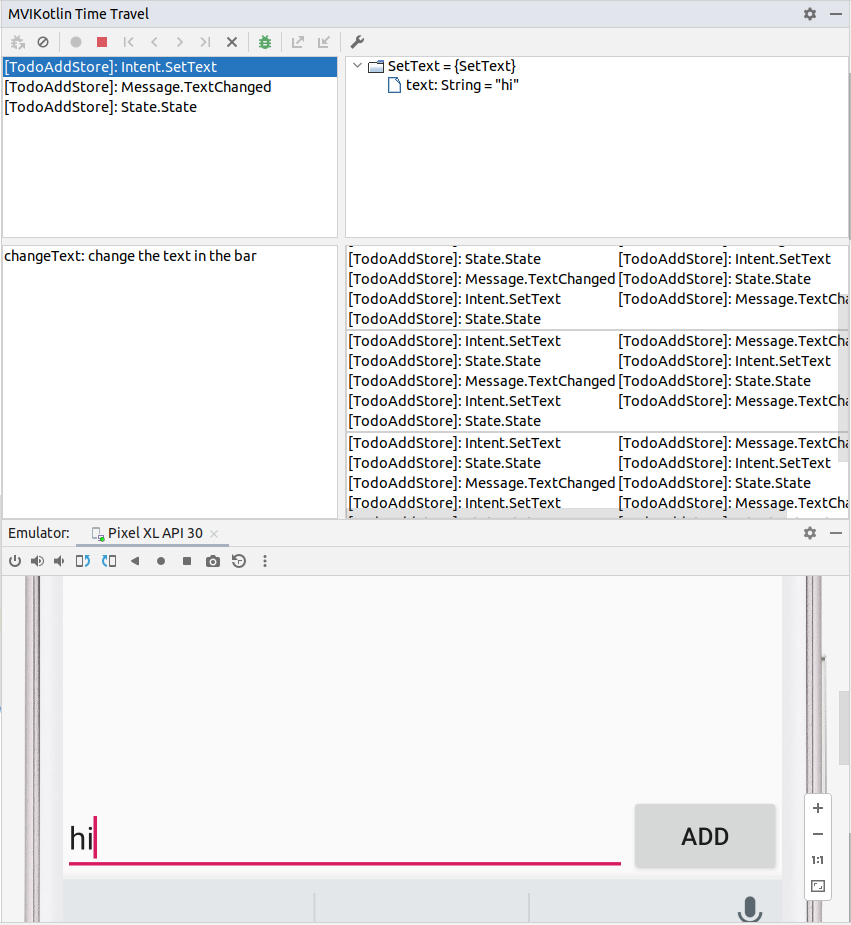
\includegraphics[height=6cm,width=10cm]{figures/plugin}
\caption{Sample view of the new plugin}
\label{fig: Sample view of the new plugin}
\end{figure}

The additions to the Intellij plugin can be described as follows:

\begin{itemize}
	\item New Panel to visualize previous events: A new panel was added to be able to visualize the events that happened. Here execution paths are shown from most recent to oldest from top to bottom. 
	\item New Panel to visualize functions that can be called in a given \textbf{intent} event: This panel displays a list of functions available to change the state of the \textbf{store}. When a function is touched, display panels will start showing for the user to insert a value for each of the parameters required to call that function.
\end{itemize}


\endinput

